\chapter{Sverdrup balance and basin-scale circulation}
\label{chap:sverdrup}

\includegraphics[width=6.5in]{figs/Geostrophic/HaidaEddy}

We saw above that the Ekman balance can drive convergences and divergences in the ocean, and that these cause the water to pile up preferentially creating pressure gradients.  The pressure gradients are then balanced by the Coriolis force, in the geostrophic balance, and water flows parallel to lines of constant pressure, clockwise around highs in the Northern hemisphere.  

This \emph{all} happens on the large scale.  If we consider the subtropical gyre, between 15 and 45 degrees, there is an Ekman convergence towards the centre of the gyre, and that causes there to be a sea-surface high there.  The water will flow around that sea-surface high in a clockwise direction (northern hemisphere).  However that leaves two questions:
\begin{enumerate}
    \item How strong will the flow be?  Alternately, how high will the highs in the middle of the gyre be?  
    \item Why is the gyre asymmetric east-west?  
\end{enumerate}

The answer is, as we will see below, that the flow is driven by the conservation of angular momentum acting in the presence of basin-scale changes in the Coriolis frequency.  Water with a negative (clockwise) torque exerted on it can either spin with negative (clockwise) angular momentum, or it can move to a region with lower background ``planetary'' angular momentum. 

\section{Circulation}

Idealizing the winds and seasurface in the subtropical gyre we have the idea that the winds blow from west to east in the westerlies (45 N) and east to west in the Trades (15 N; \fref{fig:GyreSketch}).  Based on the dynamics as we've understood them so far, this leads to an Ekman convergence everywhere in the gyre, and a raising of the seasurface height, and causing a downwelling.  

\begin{figure}[hbt]
  \begin{center}
    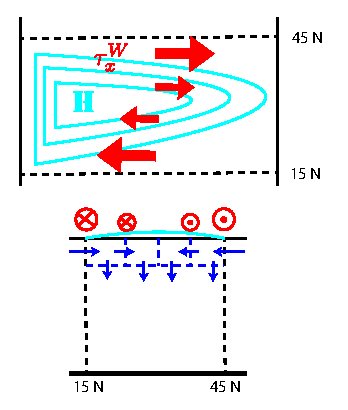
\includegraphics{figs/Sverdrup/GyreSketch}
    \caption{Idealized sketch of the wind stress in the subtropical gyre (northern hemisphere).   Top panel is from above, with coasts on the west and east side.  Westerlies peak at 45 N, and the trades at 15 N.  This makes a high in the middle, but offset to the west.  Bottom panel is the same situation looking at the side from the east towards the west. The Ekman layer is shown with the blue arrows, noting that there is downwelling throughout this gyre.}
    \label{fig:GyreSketch}  
  \end{center}
\end{figure}

However, the observed gyre is asymmetric, with the high concentrated near the western boundary. This implies that the velocity is largely equatorward everywhere in the gyre, except to the west of the high, along the \Wikiref{Western boundary}. The real situation is even more asymmetric than pictured in \fref{fig:GyreSketch}.  If we remember that the geostrophic interior velocity is proportional to the strength of the pressure gradient, then we would expect very slow flow towards the south in the interior, and very fast flow along this western boundary.  The western boundary current in the N. Pacific subtropical gyre is the \Wikiref{Kuroshio}; the \Wikiref{Gulf Stream} is the corresponding current in the Atlantic.  

\section{Conservation of potential vorticity}

The way to understand the gyre circulation is to consider the conservation of angular momentum, or in fluid mechanics we call it \Wikiref{potential vorticity}.  Just like any angular momentum, the potential vorticity changes in response to torque, in this case from the wind and seafloor.  A simplified version, useful for our case is:
\begin{equation}
    \frac{d}{dt}\left(\frac{\zeta + f}{H} \right) = \frac{1}{H^2\rho_0} \left[\frac{d\tau_y^W}{dx} - \frac{d\tau_x^W}{dy} + \frac{d\tau_y^B}{dx} - \frac{d\tau_x^B}{dy}\right]
    \label{eq:conspotvort}
\end{equation}
Here the term on the left side of the equation is the potential vorticity, and the term on the right side the torque due to the wind stress ($\tau_x^W, \tau_y^W$) and bottom friction ($\tau^B$).  $H$ is the water depth, and $f$ is the Coriolis parameter, which we keep in mind varies with latitude, or $y$.  We call this the \emph{planetary vorticity} and is the vertical angular momentum due to the earth's rotation.  
\begin{marginfigure}
    \includegraphics{figs/Sverdrup/relativevortsketch}
    \caption{Sketch of velocity gradients in a counter clockwise flow.  Note $\zeta>0$ in this flow.}
    \label{fig:relativevortsketch}  
\end{marginfigure}
The term $\zeta$ is the \Wikiref{relative vorticity} of the flow and is defined as:
\begin{equation}
    \zeta = \frac{dv}{dx} - \frac{du}{dy}
\end{equation}
where $u$ and $v$ are the x- and y-components of velocity.  It is relatively straight forward to see how this relates to a spinning flow (\fref{fig:relativevortsketch}).  Consider a flow spinning in a counter-clockwise manner.  The velocity gradients in such a flow are such that $zeta > 0$.  This uses the \Wikiref{right-hand rule}, which says that if you curl your right hand fingers in the direction of rotation, your thumb will point up for positive vorticity and down for negative vorticity (this is just a convention, and could have just as easily been the other way, but it is useful to choose one convention and stick with it).  Of course a clockwise flow has a negative vorticity.  

The same logic and sign convention applies to torque.  In the gyre sketched in \fref{fig:GyreSketch}, the gradients in $\tau^W$ are such that $\frac{d\tau_x^W}{dy} < 0$, so the wind is exerting a negative torque on the water.  


\begin{derivbox}[label={box:potentialvort}]{Derivation of potential vorticity}
Potential vorticity for a barotropic fluid is relatively straight forward to derive.  We  need the momentum equations and the continuity equation:
\begin{eqnarray*}
    \frac{du}{dt} & = & -\frac{1}{\rho}\frac{dP}{dx} + fv + \frac{1}{\rho}\frac{d\tau_x}{dz}\\
    \frac{dv}{dt} & = & -\frac{1}{\rho}\frac{dP}{dy} - fu + \frac{1}{\rho}\frac{d\tau_y}{dz}
\end{eqnarray*}
If we take $-d/dy$ of the first equation and $d/dx$ of the second and add them, then the pressure term drops out:
\begin{equation}
    \frac{d}{dt} \left( \frac{dv}{dx} - \frac{du}{dy}\right) = -f \left(\frac{du}{dx} + \frac{dv}{dy} \right) + \frac{1}{\rho}\left(\frac{d^2\tau_y}{dz\,dx} - \frac{d^2\tau_x}{dz\,dy}\right)
\end{equation}
and we note that the first term is just the derivative of $\zeta$ with time.  

We integrate this vertically from the sea-floor to sea surface, and assume that the water is $H$ deep, including any sea-surface displacements.   
\begin{equation}
    H\frac{d\zeta}{dt}  = -f H \left(\frac{du}{dx} + \frac{dv}{dy} \right) + \frac{1}{\rho}\left(\frac{d\tau_y^W}{dx} - \frac{d\tau_x^W}{dy}\right) + \frac{1}{\rho}\left(\frac{d\tau_y^B}{dx} - \frac{d\tau_x^B}{dy}\right) 
\end{equation}
So now we use the fact that $\frac{du}{dx} + \frac{dv}{dy} = -dW/dz = H^{-1}\frac{dH}{dt}$.  

TODO: finish
\end{derivbox}

We saw in the classroom demo a consequence of the conservation of potential vorticity:  when water that is initially not moving in a rotating reference frame moves from shallow water to deep water, the water column deepens, so $H$ increases (\fref{fig:PVChangeEddy}).  There are no substantial bottom or surface friction, so no external torque on the water column.  However, it does have initial \emph{planetary vorticity}, $f$ from the rotation of the reference frame.  Since there is no torque we can write:
\begin{equation}
    \frac{\zeta_0 + f_0}{H_0} = \frac{\zeta_F + f_F}{H_F} 
\end{equation}
Now initially the water is not moving, and $f$ is constant, so we can solve for $\zeta_F$ to find that the water is spinning with a vorticity that has the same sign as $f$:
\begin{equation}
    \zeta_F = f \left(\frac{H_F}{H_0} - 1 \right)
\end{equation}
\begin{marginfigure}
    \includegraphics{figs/Sverdrup/PVChangeEddy}
    \caption{Sketch of parcel of water moving from shallow to deep region.  As it moves to deep region its planetary vorticity is stretched and manifests as an eddy rotating in the same direction as the planetary vorticity.}
    \label{fig:PVChangeEddy}
\end{marginfigure}
and because $H_F>H_0$ this is a positive number.  This is all directly analogous to the spinning ice skater who draws in their arms, and makes themselves thinner, and hence spin faster, just here the effect is caused by the earth spinning rather than the skater.  \marginnote{It is actually the same math if the eddy starts spinning so it has \emph{relative vorticity} as well as having \emph{planetary vorticity}, there is just an extra term: $\zeta_F = \frac{H_F}{H_0}\left(\zeta_0 +f\right) - f$}

On the large scale, ie. our basin, it is important to bear in mind two facts.  First, $f$ varies with latitude - it is higher at the poles and zero at the equator. So that means when we think about $\frac{f+\zeta}{H}$ changing with time following a parcel of water, we need to remember that $f$ can change too.  Second, On large scales $\zeta \approx 0$, and in fact if $\zeta$ is large, like in an eddy or cyclone, it will tend to move poleward if it is a cyclone, and equatorward if an anti-cyclone.  To see why this is, consider $\zeta_0$ which is large at a latitude where $f=f_0$.  Supposing $H$ is constant, then for $\zeta_F$ to be driven to zero we have an expression for $f_F$:\marginnote{Of course a cyclone will also die out due to friction, and loss of warm water feeding the low pressure system in its centre, but the tendency to move North is because of the conservation of potential vorticity.}
\begin{equation}
    \zeta_0 + f_0 = f_F
\end{equation}
So for a hurricane $\zeta_0>0$, they always move poleward, and die out, partially because they are moving to a region with higher planetary vorticity.

\section{Sverdrup transport}  

The Sverdrup transport is a straight-forward application of the conservation of potential vorticity \fref{eq:conspotvort}, if we realize a few things.  First, let us approximate the ocean depth as a constant.  Second, we assume bottom friction is generally quite small, so $\tau_x^B\approx\tau_y^B\approx 0$. Third, note that on the scale of the whole Pacific, the relative vorticity is substantially smaller than $f$, so we can write $f+\zeta \approx f$.  To see this, consider the scale of the fastest velocity in the ocean, which is about $U\sim 1 \mathrm{m\,s^{-1}}$.  This is spread over a distance of $L\sim 10,000\ \mathrm{km}$, so the scale of vorticity is $U/L \sim 10^{-7}\ \mathrm{s^{-1}}$.  Compare to $f\approx 10^{-4}\ \mathrm{s^{-1}}$, and it is clear that on large scales (say scales > 10 km), $f>>\zeta$.  Finally, lets only consider that the wind is in the x-direction as sketched in \fref{fig:GyreSketch}.
These assumptions simplify \fref{eq:conspotvort} significantly:
\begin{equation}
    H\frac{d f}{dt} = -\frac{1}{\rho_0}\left[\frac{d\tau_y^W}{dx}\right]
\end{equation}   
So what this says is that the rate of change of $f$ is proportional to the wind torque.  In the sketch above (\fref{fig:GyreSketch}) the torque is clearly negative, so this equation says that $f$ must decrease with time following a parcel of fluid.  The way that $f$ decreases with time is by moving South because $f$ is a sinusoid centered at the equator. 

Indeed the torque tells us how fast the water will move north or south under the Sverdrup balance.  If $v$ is the north-south velocity, then 
\begin{equation}
    \frac{df}{dt} = v \frac{df}{dy}
\end{equation} 
where $y$ is in m.  $df/dy$ is a function of latitude, but we often can make the \Wikiref{beta-plane} approximation and assume its a constant $\beta$.  At 30 degrees latitude (the middle of the subtropical gyre) $\beta \approx 2.3\times 10^{-11}\ \mathrm{[(ms)^{-1}]}$.    The gives us the Sverdrup relation:
\begin{equation}
    Hv  \approx -\frac{1}{\beta \rho_0}\left[\frac{d\tau_y^W}{dx}\right]
    \label{eq:Sverdrup}
\end{equation}
So, in the case where the torque is negative the velocity $v$ is negative, and thus to the south.  

\begin{derivbox}[label={box:beta}]{Calculating Beta}
    The rate of change of $f$ with the y coordinate, $\beta = \frac{df}{dy}$ is readily calculated from $f$ and the radius of the Earth, $R$.  $f=2\Omega \sin \lambda$ and $y = R \lambda$, so  
    \begin{eqnarray*}
        \beta & = & \frac{df}{dy} \\
              & = &  \frac{df}{d\lambda} \frac{d\lambda}{dy} \\
              & = &  \frac{2\Omega}{R} \cos \lambda\  
    \end{eqnarray*}
    So with $R=6371\ \mathrm{km}$ and $2\Omega = 1.45\times10^{-4}\ \mathrm{s^{-1}}$, then at 30 N, $\beta \approx 2.3\times 10^{-11}\ \mathrm{[(ms)^{-1}]}$.  
\end{derivbox}

So let us apply to our wind torque pictured in \fref{fig:GyreSketch}.  If we assume that the wind stress profile is given by $\tau_x^W(y) = \tau_0 \sin \left(2\pi \frac{y-y_{30}}{2L}\right)$, where $\tau_0 = 0.1 \mathrm{N\,m^{-2}}$, and $L = 3300\ \mathrm{km}$ is the north-south extent of the basin (see \fref{fig:GyreWindSketch}).  So the gradient is given by 
\begin{equation}
    -\frac{d\tau_x^W}{dy} = -\tau_0 \frac{\pi}{L} \cos \pi  \left(\frac{y-y_{30}}{L}\right)
\end{equation}
So, the transport is given by 
\begin{equation}
    Hv \approx \left(4.14 \ \mathrm{m^2\,s^{-1}}\right) \cos \pi  \left(\frac{y-y_{30}}{L}\right)
\end{equation}
So, at 30-degrees, the 2-D transport is $4.14\ \mathrm{m^2\,s^{-1}}$. Averaged over the 4000-m water depth we can arrive at an average velocity of $v\approx 1\ \mathrm{mm\, s^{-1}}$, though the actual wind-driven transport tends to be surface intensified.  Integrated across the Pacific, with a width of 10,000 km this yields a total 3-D transport of $4.14\times10^{7}\ \mathrm{m^3\,s^{-1}}$, or 40 Sv.  Note that as we get closer to the bottom ($\lambda=15 N$) and the top ($\lambda= 45N$) the transport drops to zero (\fref{fig:GyreSketch}). 
\begin{figure}[hbt]
  \begin{center}
    \includegraphics{figs/Sverdrup/GyreWindSketch}
    \caption{Sketch of shape of wind stress (left), shape of Sverdrup transport (middle), and arrows indicating what that transport looks like when looking from above (right).}
    \label{fig:GyreWindSketch}  
  \end{center}
\end{figure}

Note that this sense of transport agrees with observations of a sea-surface high displaced to the west of the gyre.  Of the flow is clockwise around the high, then all the water to the east of the high will be moving southwards.  This estimate also accords with our best estimates of the transport in the gyre from calculating geostrophic velocities (\fref{GrayRiserFig2}).  

\begin{figure}[hbt]
  \begin{center}
    \includegraphics{figs/Sverdrup/GrayRiserFig2}
    \caption{Geostrophic streamfunction at 5 dbar in $m^2s^{-2}$, estimated from Argo floats. Red high, clockwise flow. \citep{grayriser14}}
    \label{fig:GrayRiserFig2}  
  \end{center}
\end{figure}

\subsection{Alternative derivation: Ekman pumping}

An alternative way to think about the Sverdrup balance is to separate the upper-ocean Ekman layer from the interior of the ocean.  In this case, the interior of the ocean does not feel the wind friction, and hence has no mechanical torque acting on it.  However, there is a constant downwelling of water from the Ekman pumping.  This causes the water already in the interior to be squished, so $dH/dt < 0$, and the water will tend to move south.

In terms of the vorticity equation, we can write it with no torques and small relative vorticity as 
\begin{equation}
    \frac{d}{dt}\frac{f}{H} = 0
\end{equation}
or using the the fact that $d(ab)/dt = adb/dt + b da/dt$:
\begin{equation}
    Hv\beta = f \frac{dH}{dt} = f w
\end{equation}
where the rate of squishing of the deeper water is $w$, the rate of Ekman pumping (\fref{fig:SverdrupEkman}).  

\begin{figure}[hbt]
  \begin{center}
    \includegraphics{figs/Sverdrup/SverdrupEkman}
    \caption{Sketch of how Ekman pumping pushes down on the water in the interior, causing $H$ to decrease, and hence the water to tend to flow south to compensate.}
    \label{fig:SverdrupEkman}  
  \end{center}
\end{figure}

We noted in \fref{ch:coriolis} that the rate of Ekman pumping is related the to curl of the wind stress:
\begin{equation}
    w = -\frac{1}{f\rho_0}\frac{d\tau_x^W}{dy}
\end{equation}
or, 
\begin{equation}
    Hv\beta = f \frac{dH}{dt} = -\frac{1}{\rho_0}\frac{d\tau_x^W}{dy}
\end{equation}
just like in the derivation above. 


\section{Return flow}

Remember that the Sverdrup balance applies from the top to the bottom of the water column, so if all the water between 15 and 45 N is flowing south under the Sverdrup balance, there has to be a return flow to the north somewhere.  The shape of the sea-surface height in \fref{fig:GrayRiserFig2} indicates that the northward flow is on the west side of the basin, and indeed we can easily argue that this is indeed true.  

In order for flow to move north, it needs a positive torque.  The wind torque is negative, so the opposing torque must be from friction and tend to spin the water counter-clockwise.  If we assume the torque comes from the sides, we simply cheque the sign of the torque exerted by a parcel of water moving north on either sidewall (\fref{fig:TorquesReturn}).  If the return flow were in the east, then the friction force would be on the east side of a parcel of water, and there would be no friction force on the left side.  This would tend to spin the water in a clockwise sense, or with negative torque.  This is, of course, the wrong sense, because we need a positive torque.  If we consider a return flow on the west side, the friction is on the west side of a parcel moving north, and there is no friction on the east side, so the parcel will tend to be torqued in a counter-clockwise direction, and hence this is where the return flow must be.  

\begin{figure}[hbt]
  \begin{center}
    \includegraphics{figs/Sverdrup/TorquesReturn}
    \caption{Sketch of sidewall torque on two alternate return flows in a subtropical gyre.}
    \label{fig:TorquesReturn}  
  \end{center}
\end{figure}

The final missing piece is that water must move fro the interior to and from the western boundary current.  just using conservation of volume, we can readily infer that the water south of 30 N must be moving west, and the water north must be moving east.  Thus the flow follows the geostrophic contours as plotted in \fref{fig:GrayRiserFig2}, moving around the high sealevel in a clockwise fashion.  Where the sea level gradient is steepest, the flow is the fastest, in the Western Boundary current.  

Looking at \fref{fig:GrayRiserFig2}, it is apparent that there is a western boundary current in both the northern and southern hemispheres, and in all the ocean basins.  In the subtropical gyres, these currents carry water from the equator towards the poles, and in the subpolar gyres, they do the opposite.  Its worth testing your knowledge by considering the wind patterns in the southern hemisphere, or the subpolar gyre, and see if the sign of the torque accords with \fref{fig:GrayRiserFig2}. 




 